\section{\rqtwo}



Our second research question investigates the differences between program variants at runtime.
To answer RQ2, we execute each program/variant to collect their execution traces and execution times.
For each programs' population we compare \autoref{metric:stack} and \autoref{metric:time} for each program/variant pair.
This section is organized as follows. First, we analyze the programs' populations by comparing the values of \autoref{metric:stack} for each pair of program/variant. The pairwise comparison will hint at the results at the population level. We want to analyze not only the differences of a variant regarding its original program, but we also want to compare the variants against other variants. Second, we do the same pairwise strategy for \autoref{metric:time}, performing a Mann-Withney U test for each pair of program/variant times distribution. Finally, we conclude and answer RQ2.

\subsection*{stack operation traces.}

% Describe the first figure
In \autoref{rq2:dtw_distrib} we plot the distribution of all \DTW comparisons for all pairs of program/variant of each program's population generated un RQ1. All compared programs are statically different. Each vertical violin plot (in logarithmic scale) represents the \DTW values for a program of the \corpusrosetta corpus for which we generated variants. For illustration, we exclude those programs with only one variant. The X-axis is sorted in descending order of the size of the program's population. We want to remark that the programs excluded from the plot all result from their comparisons in \DTW larger than zero. Thus, the unique generated variants present a different behavior in terms of stack operation traces.


% Main insight
We have observed that in the majority of the cases, the mean of the comparison values is huge in all cases. We analyze the length of the traces, and one reason behind such large values of \DTW is that some variants result from constant inferring. For example, if a loop is replaced by a constant, instead of several symbols in the stack operation trace, we observe one. Consequently, the distance between two program traces is significant. We have observed no relation between how aggressive the transformation is and the length of the traces.  

In some cases, even when the variants are statically different, two programs/variants result in a \DTW value oz zero, \ie they result in the same stack operation trace. We identified two main reasons behind this phenomenon. First, the code transformation that generates the variant targets a non-executed or dead code. This result calls for future work on correct code debloating \citationneeded. Second, some variants have two different instructions that trigger the same stack operations. For example, the code replacements below illustrate the case. The four cases leave the same value in the stack operation trace.

\begin{code}[H]
\centering
\noindent\begin{minipage}{.23\linewidth}
\lstdefinestyle{nccode2}{
    numbers=none,
    firstnumber=1,
    stepnumber=1,
    numbersep=10pt,
    tabsize=4,
    showspaces=false,
    breaklines=true, 
    showstringspaces=false,
    moredelim=**[is][{\btHL[fill=black!10]}]{`}{`},
    moredelim=**[is][{\btHL[fill=celadon!40]}]{!}{!}
}
    \lstset{
        language=WAT,
        style=nccode2,
        basicstyle=\footnotesize\ttfamily,
        columns=fullflexible,
        breaklines=true
    }
    \begin{lstlisting}
(1) `i32.lt_u`
(2) `i32.le_s`
    \end{lstlisting}
\end{minipage}\hfill%
\noindent\begin{minipage}{0.2\linewidth}
\lstdefinestyle{nccode2}{
    numbers=none,
    firstnumber=1,
    stepnumber=1,
    numbersep=10pt,
    tabsize=4,
    showspaces=false,
    breaklines=true, 
    showstringspaces=false,
    moredelim=**[is][{\btHL[fill=black!10]}]{`}{`},
    moredelim=**[is][{\btHL[fill=celadon!40]}]{!}{!}
}

    \lstset{
        language=WAT,
        style=nccode2,
        basicstyle=\footnotesize\ttfamily,
        columns=fullflexible,
        breaklines=true
    }
    \begin{lstlisting}
!i32.lt_s!
!i32.lt_u!
    \end{lstlisting}
\end{minipage}\hfill%
\noindent\begin{minipage}{.3\linewidth}
\lstdefinestyle{nccode2}{
    numbers=none,
    firstnumber=1,
    stepnumber=1,
    numbersep=10pt,
    tabsize=4,
    showspaces=false,
    breaklines=true, 
    showstringspaces=false,
    moredelim=**[is][{\btHL[fill=black!10]}]{`}{`},
    moredelim=**[is][{\btHL[fill=celadon!40]}]{!}{!}
}

    \lstset{
        language=WAT,
        style=nccode2,
        basicstyle=\footnotesize\ttfamily,
        columns=fullflexible,
        breaklines=true
    }
    \begin{lstlisting}
(3) `i32.ne`
(4) `local.get 6`
    \end{lstlisting}
\end{minipage}\hfill%
\noindent\begin{minipage}{0.2\linewidth}
\lstdefinestyle{nccode2}{
    numbers=none,
    firstnumber=1,
    stepnumber=1,
    numbersep=10pt,
    tabsize=4,
    showspaces=false,
    breaklines=true, 
    showstringspaces=false,
    moredelim=**[is][{\btHL[fill=black!10]}]{`}{`},
    moredelim=**[is][{\btHL[fill=celadon!40]}]{!}{!}
}

    \lstset{
        language=WAT,
        style=nccode2,
        basicstyle=\footnotesize\ttfamily,
        columns=fullflexible,
        breaklines=true
    }
    \begin{lstlisting}
!i32.lt_u!
!local.get 4!
    \end{lstlisting}
\end{minipage}
\end{code}


\begin{figure*}[h]
    \centering
    \hspace*{-0.1\linewidth}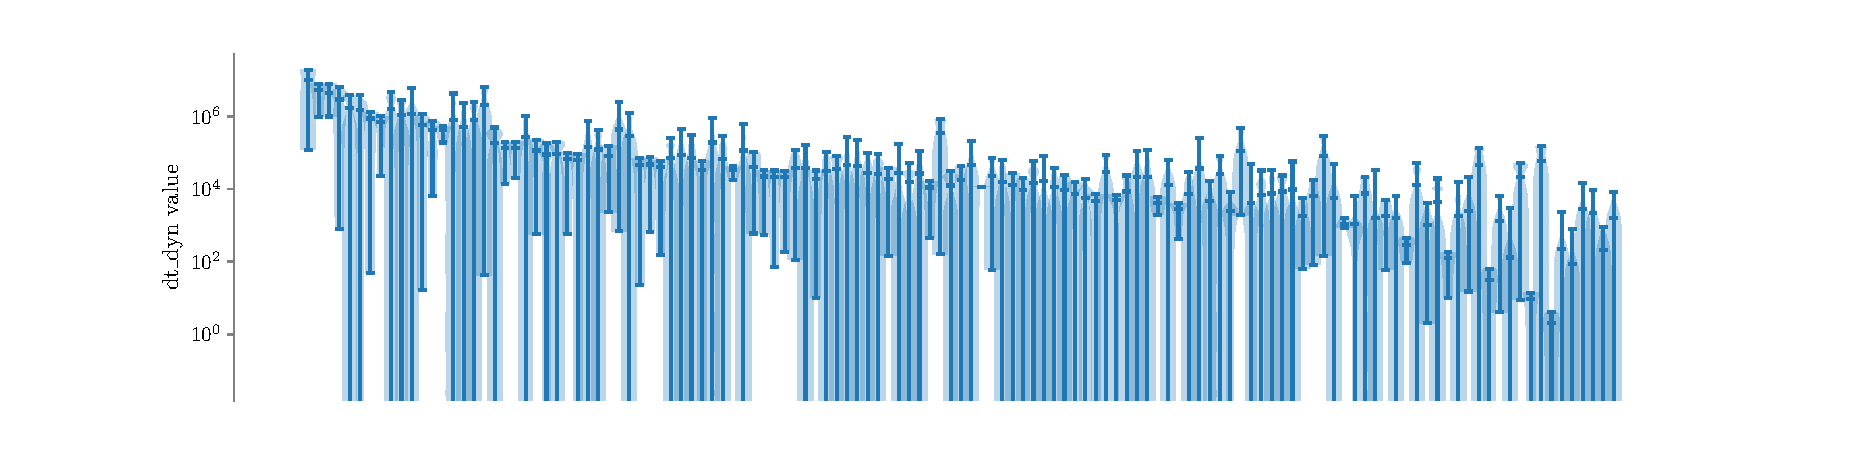
\includegraphics[width=1.2\linewidth]{plots/dtw_distrib.pdf}
    \caption{Pairwise of \autoref{metric:stack} values in logarithmic scale. Each vertical plot represents a program and its variants. The plot only contains the programs for which we generate more than one variant, \ie more than one pair of programs comparisons. }
    \label{rq2:dtw_distrib}
\end{figure*}

In \autoref{rq2:zero_ratio} we plot those programs for which at least one comparison (\DTW) is zero. The plot contains 82 vertical bars, one for each program. In the other cases, all \DTW values are non-zero. We can observe that even when some programs/variants result in the same trace, there is no case for which all variants return the same stack operation trace with all bars above $Y=0.2$. There is always at least one generated variant that is dynamically different from the original program. 

\newcommand{\zerocountprogs}{82\xspace}

\begin{figure*}[h]
    \centering
    \hspace*{-0.1\linewidth}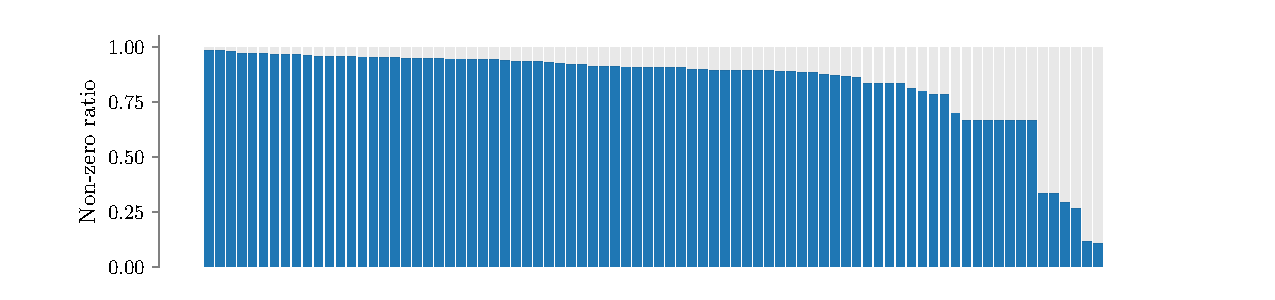
\includegraphics[width=1.2\linewidth]{plots/non_zero_ratio.pdf}
    \caption{ Ratio of \autoref{metric:stack} with non-zero values for each program's population. Each vertical line represents the number of \DTW different from zero in a pairwise comparison of each program and its variants. The plot only contains the \zerocountprogs/239  with at least one pair comparison with zero value.}
    \label{rq2:zero_ratio}
\end{figure*}

\subsection*{Execution times.}

% Overall results
For each program's population, we compare the execution time distributions, \autoref{metric:time}, of each pair of program/variant.
Overall diversified programs, 169 out of 239 have at least one variant with a different execution time distribution than the original program (P-value $<$ $0.01$ in the Mann-Withney test). This result shows that we effectively generate variants that yield significantly different execution times.

By analyzing the data, we observe the following trends. First, if our tool infers control-flows as constants in the original program, the variants execute faster than the original, sometimes by one order of magnitude. On the other hand, if the code is augmented with more instructions, the variants tend to run slower than the original. 

In both cases, we generate a variant with a different execution time than the original. Both cases are good from a randomization perspective since this minimizes the certainty a malicious user can have about the program's behavior. Therefore, a deeper analysis of how this phenomenon can be used to enforce security will be discussed in answering RQ3.

To better illustrate the differences between executions times in the variants, we dissect the execution time distributions for two programs' populations. 
% describe figures
The plots in \autoref{rq3:perf} show the execution time distributions of programs \texttt{Base64\_decode} and \texttt{Hilbert\_curve} and their variants. 
We illustrate time diversification with these two programs because, for both, we generate unique variants with all types of transformations previously discussed in \autoref{results:rq1}.
In the plots along the X-axis, each vertical set of points represents the distribution of 100 execution times per program/variant. The Y-axis represents the execution time value in milliseconds. The original program is highlighted in magenta color: the distribution of 100 execution times is given on the left-most part of the plot, and its median execution time is represented as a horizontal dashed line. The median execution time is represented as a blue dot for each execution time distribution, and the vertical gray lines represent the entire distribution. The bolder gray line represents the 75\% interquartile. The program variants are sorted concerning the median execution time in descending order.



\begin{figure*}[h]
    \centering
    \hspace*{-0.05\linewidth}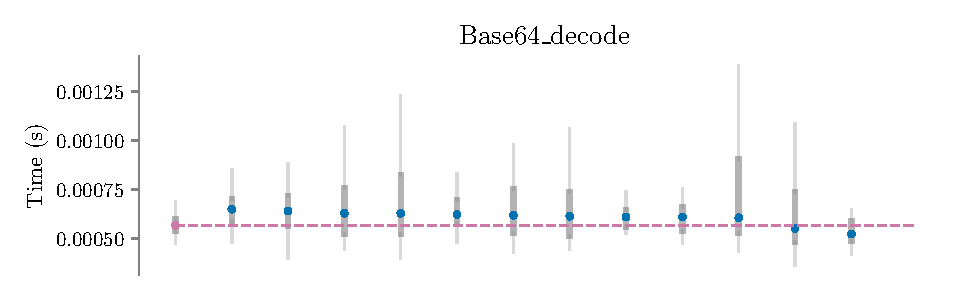
\includegraphics[width=1.1\linewidth]{plots/base64.pdf}
    \hspace*{-0.05\linewidth}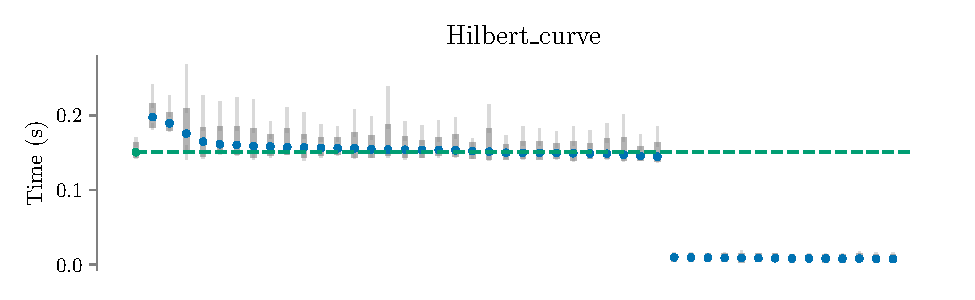
\includegraphics[width=1.1\linewidth]{plots/hilbert_curve.pdf}
    \caption{Execution time distributions for \texttt{Base64\_decode} and \texttt{Hilbert\_curve} program and their variants in top and bottom figures respectively. Baseline execution time mean is highlighted with the magenta horiontal line. }
    \label{rq3:perf}
\end{figure*}

% explanation
For \texttt{Base64\_decode}, the majority of variants are constantly slower than the reference programs (blue dot above the magenta line). For \texttt{Hilbert\_curve}, many diversified variants are optimizations (blue dots below the magenta bar). The case of \texttt{Hilbert\_curve} is graphically clear, and the last third represents faster variants resulting from code transformations that optimize the original program.
Our tool provides program variants in the whole spectrum of time executions, lower and faster variants than the original program. The developer is in charge of deciding the trade-off between taking all variants or only the ones providing the same or less execution time for the sake of less overhead. 

\section{Answer to RQ2.}
We empirically demonstrate that our approach generates program variants for which their execution traces are different. We stress the importance of complementing static and dynamic studies of programs variants. For example, if two programs are statically different, that does not necessarily mean different runtime behavior. There is at least one generated variant for all executed programs that provides a different execution trace. 
% answer to RQ2
We generate variants that exhibit a significant diversity of execution times. For example, for $169/239\,(71\%)$ of the diversified programs, at least one variant has an execution time distribution that is different compared to the execution time distribution of the original program. 
The result from this study encourages the composition of the variants to provide a more resilient execution.